% !TEX encoding = UTF-8 Unicode

\documentclass[oneside]{book}

%%%%%%%%%%%%%%%%%%%%%%%%%%%%%%%%%%%%%%%%%%%%%
% PACKAGES
%%%%%%%%%%%%%%%%%%%%%%%%%%%%%%%%%%%%%%%%%%%%%

% STANDARD

\usepackage{etoolbox}
\usepackage{subcaption}
\usepackage{float}
\usepackage{xparse}
\usepackage{xstring}
\usepackage{enumitem}
\usepackage{graphicx}
\usepackage{diagbox}
\usepackage{listings}
\usepackage{rotating} %sideways environment

% PROOF READING

\usepackage[T1]{fontenc}
\usepackage[utf8]{inputenc}
\usepackage[english]{babel}

% URL WITHIN THE PDF

\usepackage{hyperref}

% BIBLIOGRAPHY

\usepackage[nottoc,numbib]{tocbibind}

% TABLES

\usepackage{booktabs}
\usepackage{makecell}



% SYMBOLS

\usepackage{pifont}
\usepackage{fontawesome}
\usepackage{textcomp} %TM

% URL

\usepackage{url}

% WARNING NOTES

\usepackage{mdframed}





% TIKZ

\usepackage{tikz}
\usetikzlibrary{arrows.meta, matrix, arrows,automata,positioning}

% FONTS AND COLORS

\usepackage{xcolor}
\usepackage{cancel}

% THEOREMS & MATHS

\usepackage{amsmath}
\usepackage{amsthm}
\usepackage{amssymb}
\usepackage{mathtools}

% ALGORITHMS

\usepackage[ruled,vlined,linesnumbered]{algorithm2e}

% GLOSSARIES

\usepackage[toc,acronym,style=index]{glossaries}
\usepackage[postdot]{glossaries-extra}

%%%%%%%%%%%%%%%%%%%%%%%%%%%%%%%%%%%%%%%%%%%%%
% IMPORTS OF CUSTOM COMMANDS
%%%%%%%%%%%%%%%%%%%%%%%%%%%%%%%%%%%%%%%%%%%%%

% !TEX encoding = UTF-8 Unicode

\newcommand{\edot}{%
    ë%
    %{\"{e}}%
}

\newcommand{\e}{%
    ë%
    %{{\"e}}%
}

% param 1 italian
% param 2 albanian
\newcommand{\addTranslation}[4][]{%
    % FORM ITALIAN TO ALBANIAN
    \newglossaryentry{#1}%
    {%
        type={itan},%
        name={#1},%
        description={#2}%
    }%
    %
    % FORM ALBANIAN TO ITALIAN
    \newglossaryentry{#2}%
    {%
        type={anit},%
        name={#2},%
        description={#1}%
    }%
}

\NewDocumentCommand{\addTranslationRow}{m}{%
    {#1} & \Glsdesc{#1}%
}
\usepackage{calculator}

%%%%%%%%%%%%%%%%%%%%%%%%%%%%%%%%%%%%%%%%%%%%%
% REFERENCES
%%%%%%%%%%%%%%%%%%%%%%%%%%%%%%%%%%%%%%%%%%%%%

\makeatletter

% Add a reference to a section
% param1 the label of the section
\NewDocumentCommand{\lstref}{m}{%
    Listing \ref{#1}%
}

% Add a reference to a section
% param1 the label of the section
\NewDocumentCommand{\listingref}{m}{%
    Listing \ref{#1}%
}


% Add a reference to a subsubsection
% param1 the label of the subsubsection
\NewDocumentCommand{\subsubsectionref}{m}{%
    Sub Sub Section \ref{#1}%
}

% Add a reference to a section
% param1 the label of the section
\NewDocumentCommand{\sectionref}{m}{%
    Section \ref{#1}%
}

% Add a reference to a equation
% param1 the label of the equation
\NewDocumentCommand{\equationref}{m}{%
    Equation \eqref{#1}%
}

% Add a reference to a algorithm line
% param1 the label of the algorithm line
\NewDocumentCommand{\alglineref}{m}{%
    Line \ref{#1}%
}

% Add a reference to a algorithm line
% param1 the label of the algorithm where piece starts
% param1 the label of the algorithm where priece ends
\NewDocumentCommand{\alglinesref}{m m}{%
    Lines \ref{#1}--\ref{#2}%
}

% Add a reference to an algorithm
% param1 the label of the algorithm
\NewDocumentCommand{\algref}{m}{%
    Algorithm \ref{#1}%
}

% Add a reference to a definition
% param1 the label of the definition
\NewDocumentCommand{\defref}{m}{%
    Definition \ref{#1}%
}

% Add a reference to a definition
% param1 the label of the first definition
% param2 the label of the second definition
\NewDocumentCommand{\defsref}{m m}{%
    Definitions \ref{#1}--\ref{#2}%
}

% Add a reference to a figure
% param1 the label of the figure
\NewDocumentCommand{\figref}{m}{%
    Figure \ref{#1}%
}

% Add a reference to a range of figure
% param1 the label of the first figure in the range (inclusive)
% param2 the label of the last figure in the range (inclusive)
\NewDocumentCommand{\figsref}{m m}{%
    Figures \ref{#1}--\ref{#2}%
}


\NewDocumentCommand{\r@figrefs}{m}{%
    \@ifnextchar\bgroup{, \ref{#1}\r@figrefs}{ and \ref{#1}}%
}
% Add a reference to a figure
% param1 the label of the figure
\NewDocumentCommand{\figrefs}{m}{%
    Figures \ref{#1}\r@figrefs%
}

% Add a reference to a table
% param1 the label of the table
\NewDocumentCommand{\tblref}{m}{%
    Table \ref{#1}%
}

% Add a reference to a theorem
% param1 the label of the table
\NewDocumentCommand{\thmref}{m}{%
    Theorem \ref{#1}%
}

% Add a reference to a lemma
% param1 the label of the lemma
\NewDocumentCommand{\lemmaref}{m}{%
    Lemma \ref{#1}%
}

% Add a reference to an example
% param1 the label of the example
\NewDocumentCommand{\exampleref}{m}{%
    Example \ref{#1}%
}

%%%%%%%%%%%%%%%%%%%%%%%%%%%%%%%%%%%%%%%%%%%%%
% EXAMPLE
%%%%%%%%%%%%%%%%%%%%%%%%%%%%%%%%%%%%%%%%%%%%%

\theoremstyle{definition}
\newtheorem{example}{Example}[section]

%%%%%%%%%%%%%%%%%%%%%%%%%%%%%%%%%%%%%%%%%%%%%
% USEFUL COMMANDS
%%%%%%%%%%%%%%%%%%%%%%%%%%%%%%%%%%%%%%%%%%%%%

%DOES NOT WORK
\NewDocumentEnvironment{verticalAlign}{+b}{%
    \topskip0pt%
    \vspace*{\fill}%
    {#1}%
    \vspace*{\fill}%
}{%
}

% Indent a body of text
% param1 dimension representing the space you want to indent
% param2 body actual content to put in the indented wall of text
\NewDocumentEnvironment{indentText}{O{3cm} +b}{%
    \begin{minipage}{\dimexpr\textwidth-#1}%
        #2%
        \xdef\tpd{\the\prevdepth}%
    \end{minipage}%
}{%
}

% Put a definition block in the text
%
% param1 the definition name. If not specified we won't have a definition
% param2 the label we want this definition to have. Input of \label. If not specified we won't put the \label command
% param3 the content of the definition
% \NewDocumentEnvironment{definition}{o o +b}{%
%     %BEGIN
%     \IfNoValueTF{#1}{%
%         \begin{theorem}%
%     }{%
%         \begin{theorem}[#1]%
%     }%
%     \IfNoValueF{#2}{%
%         \label{#2}%
%     }%
%     #2%
%     \end{theorem}%
% }{%
%     %END
% }
%     \IfNoValueTF{#1}{%
%         \begin{theorem}
%     }{%
%     }%
% }

\NewDocumentCommand{\setFontSize}{m o m}{%
    \IfNoValueF{#2}{%
        \fontsize{#1}{#2}\selectfont#3%
    }{%
        % see https://texblog.org/2012/08/29/changing-the-font-size-in-latex/
        \MULTIPLY{#1}{1.2}{\setFont@baseline}%
        \fontsize{#1}{\setFont@baseline}\selectfont#3%
    }%
}

% Adds a todo embedded in the text (colored blue)
% param1: an optional star: if a star is present, we will put the todo as a footnote
% param2: the text to put
\NewDocumentCommand{\todo}{s m}{%
    \IfBooleanTF{#1}{%
        \footnote{\color{blue} #2}%
    }{%
        {\color{blue} #2}%
    }%
}

%Adds a todo as a footnoe
\NewDocumentCommand{\code}{m}{%
    \texttt{#1}%
}

% draw a square.
% param1: fill color red!50
% param2: border color (default to black)
\NewDocumentCommand{\drawFilledSquare}{m O{black}}{%
    \begin{tikzpicture}%
        \node [rectangle,draw={#2},fill={#1}] (m) at (0,0) {};%
    \end{tikzpicture}%
}

% print a computer science ordered pair
% param1 first element of the pair
% param2 second element of the pair
\NewDocumentCommand{\paircs}{m m}{%
    \wrapMath{\langle {#1}, {#2} \rangle }%
}

\NewDocumentEnvironment{coloredBlock}{m O{blue} O{white}}{%
\setbeamercolor{block title}{bg=#2, fg=#3}
    \begin{block}{#1}%
}{%
    \end{block}%
}

\NewDocumentCommand{\stacksymbols}{m m}{%
    \wrapMath{\stackrel{\mathclap{#1}}{#2}}%
}

\NewDocumentCommand{\bigO}{m}{%
    \wrapMath{\mathcal{O}(#1)}%
}

\NewDocumentCommand{\nil}{}{%
    \texttt{NIL}%
}

\NewDocumentCommand{\doublePlus}{}{%
    \ifmmode{+\!\!+}\else{$+\!\!+$}\fi%
}

\NewDocumentCommand{\isInMath}{m m}{%
    \ifmmode{#1}\else{#2}\fi%
}

\NewDocumentCommand{\wrapMath}{m}{%
    \ifmmode{#1}\else{$#1$}\fi%
}

%apply double quotes on the parameter
% param1 the text to wrap quote
\NewDocumentCommand{\dquote}{m}{%
    ``{#1}''%
}

\NewDocumentCommand{\squote}{m}{%
    \isInMath%
        {\mbox{`}{#1}\mbox{'}}%
        {`{#1}'}%
}

%%%%%%%%%%%%%%%%%%%%%%%%%%%%%%%%%%%%%%%%%%%%%
% SYMBOLS
%%%%%%%%%%%%%%%%%%%%%%%%%%%%%%%%%%%%%%%%%%%%%

% draw a "v" representing a checkbox which has been checked
\NewDocumentCommand{\checked}{}{%
\tikz\fill[scale=0.4](0,.35) -- (.25,0) -- (1,.7) -- (.25,.15) -- cycle;%
}

% draw a "x" representing a checkbox which has been checked
\NewDocumentCommand{\unchecked}{}{%
\tikz\fill[scale=0.4]%
    (-0.35,+0.35) -- (+0.00,+0.07) --%
    (+0.40,+0.40) -- (+0.07,+0.00) --%
    (+0.35,-0.35) -- (+0.00,-0.07) --%
    (-0.40,-0.40) -- (-0.07,+0.00) --%
    cycle;%
}

%%%%%%%%%%%%%%%%%%%%%%%%%%%%%%%%%%%%%%%%%%%%%
% ACRONYM
%%%%%%%%%%%%%%%%%%%%%%%%%%%%%%%%%%%%%%%%%%%%%

\NewDocumentCommand{\eg}{}{%
    e.g.,%
}

\NewDocumentCommand{\ie}{}{%
    i.e.,%
}

\NewDocumentCommand{\st}{}{%
    s.t.%
}

\NewDocumentCommand{\wrt}{}{%
    w.r.t.%
}
\RenewDocumentCommand{\iff}{}{%
    \textit{iff}%
}

% see https://tex.stackexchange.com/a/369691/145331
\let\@oldcite\cite
\renewcommand*\cite[1]{~\@oldcite{#1}}


\makeatother

% Commands which are just alias for common latex operations

%%%%%%%%%%%%%%%%%%%%%%%%%%%%%%%%%%%%%%%%%%%%%
% WARNING AND NOTES
%%%%%%%%%%%%%%%%%%%%%%%%%%%%%%%%%%%%%%%%%%%%%

% Show an attention box. The body of the environment is the body of the box 
\NewDocumentEnvironment{attention}{}{%
    \par%
        \begin{mdframed}[linewidth=3pt,linecolor=red]%
            \begin{list}{}{\leftmargin=1cm \labelwidth=\leftmargin}%
                \item[\Large\faBomb]%
}{%
            \end{list}%
        \end{mdframed}%
    \par
}

% Show a warning box. The body of the environment is the body of the box
\NewDocumentEnvironment{warning}{}{%
    \par%
        \begin{mdframed}[linewidth=3pt,linecolor=orange]%
            \begin{list}{}{\leftmargin=1cm \labelwidth=\leftmargin}%
                \item[\Large\faWarning]%
}{%
            \end{list}%
        \end{mdframed}%
    \par
}

% Show an note box. The body of the environment is the body of the box
\NewDocumentEnvironment{info}{}{%
    \par%
        \begin{mdframed}[linewidth=3pt,linecolor=blue]%
            \begin{list}{}{\leftmargin=1cm \labelwidth=\leftmargin}%
                \item[\Large\faBook]%
}{%
            \end{list}%
        \end{mdframed}%
    \par
}

% Alias of "info"
\NewDocumentEnvironment{note}{}{%
    \par%
        \begin{mdframed}[linewidth=3pt,linecolor=blue]%
            \begin{list}{}{\leftmargin=1cm \labelwidth=\leftmargin}%
                \item[\Large\faBook]%
}{%
            \end{list}%
        \end{mdframed}%
    \par
}

%%%%%%%%%%%%%%%%%%%%%%%%%%%%%%%%%%%%%%%%%
% FLOATS
%%%%%%%%%%%%%%%%%%%%%%%%%%%%%%%%%%%%%%%%%

%Setup the a horizontal page instead of the classic portait page
\NewDocumentCommand{\insertFigure}{}{}
\NewDocumentEnvironment{horizontalpage}{+b}{%
    \begin{sidewaysfigure}%
        #1%
    \end{sidewaysfigure}%
}{%
}

%%%%%%%%%%%%%%%%%%%%%%%%%%%%%%%%%%%%%%%%%
% TEX COMMONS
%%%%%%%%%%%%%%%%%%%%%%%%%%%%%%%%%%%%%%%%%

% Write something in italic. Alias of \textit
% param1 the text to write in italic
\NewDocumentCommand{\italic}{m}{%
    \textit{#1}%
}

%%%%%%%%%%%%%%%%%%%%%%%%%%%%%%%%%%%%%%%%%
% GLOSSARIES
%%%%%%%%%%%%%%%%%%%%%%%%%%%%%%%%%%%%%%%%%

% Display the given acronym 
% param1 name of the acronym to print
\NewDocumentCommand{\acronymRef}{m}{%
   \gls{#1}%
}


% Display the given acronym 
% param1 name of the acronym to print
\NewDocumentCommand{\acrref}{m}{%
   \gls{#1}%
}

% Display a glossary entry with the first letter as miniscule.
%This is just a more rememberable alias of \gls
% param1 name of the glossary entry to cite. 
\NewDocumentCommand{\glossaryRef}{m}{%
    \gls{#1}%
}

% Display a glossary entry with the first letter as capital.
%This is just a more rememberable alias of \Gls
% param1 name of the glossary entry to cite. 
\NewDocumentCommand{\GlossaryRef}{m}{%
    \Gls{#1}%
}

% Display a glossary entry with the first letter as miniscule.
%This is just a more rememberable alias of \gls
% param1 name of the glossary entry to cite. 
\NewDocumentCommand{\glsref}{m}{%
    \gls{#1}%
}

% Display a glossary entry with the first letter as capital.
%This is just a more rememberable alias of \Gls
% param1 name of the glossary entry to cite. 
\NewDocumentCommand{\Glsref}{m}{%
    \Gls{#1}%
}



%%%%%%%%%%%%%%%%%%%%%%%%%%%%%%%%%%%%%%%%
% NAMES
%%%%%%%%%%%%%%%%%%%%%%%%%%%%%%%%%%%%%%%%

\NewDocumentCommand{\true}{}{%
    \code{true}%
}

\NewDocumentCommand{\false}{}{%
    \code{false}%
}

\NewDocumentCommand{\NPComplete}{}{%
    \code{NP}-Complete%
}

\NewDocumentCommand{\NPHard}{}{%
    \code{NP}-Hard%
}

\NewDocumentCommand{\NPHardness}{}{%
    \code{NP}-Hardness%
}

%define default listing settings

\lstset{%
    postbreak=\mbox{\textcolor{red}{$\hookrightarrow$}\space},%
    frame={single},%
    breaklines={true},%
    captionpos={b}%
}

%%%%%%%%%%%%%%%%%%%%%%%%%%%%%%%%%%%%%%%%%%
% XML
%%%%%%%%%%%%%%%%%%%%%%%%%%%%%%%%%%%%%%%%%%

\definecolor{xmlgray}{rgb}{0.4,0.4,0.4}
\definecolor{xmldarkblue}{rgb}{0.0,0.0,0.6}
\definecolor{xmlcyan}{rgb}{0.0,0.6,0.6}


\lstdefinelanguage{xml}{
  basicstyle=\footnotesize\ttfamily,
  columns=fullflexible,
  showstringspaces=false,
  commentstyle=\color{xmlgray}\upshape,
    %
  morestring=[b]",
  morestring=[s]{>}{<},
  morecomment=[s]{<?}{?>},
  stringstyle=\color{black},
  identifierstyle=\color{xmldarkblue},
  keywordstyle=\color{xmlcyan},
  morekeywords={xmlns,version,type}% list your attributes here
}

%%%%%%%%%%%%%%%%%%%%%%%%%%%%%%%%%%%%%%%%%%
% JSON
%%%%%%%%%%%%%%%%%%%%%%%%%%%%%%%%%%%%%%%%%%

%define listing for json language
% see https://tex.stackexchange.com/a/433961/145331
\definecolor{eclipseStrings}{RGB}{42,0.0,255}
\definecolor{eclipseKeywords}{RGB}{127,0,85}
\colorlet{numb}{magenta!60!black}

\lstdefinelanguage{json}{
    basicstyle=\footnotesize\ttfamily,
    commentstyle=\color{eclipseStrings}, % style of comment
    stringstyle=\color{eclipseKeywords}, % style of strings
    numbers=left,
    numberstyle=\scriptsize,
    stepnumber=1,
    numbersep=8pt,
    showstringspaces=false,
    breaklines=true,
    frame={single},
    %backgroundcolor=\color{gray}, %only if you like
    string=[s]{"}{"},
    comment=[l]{:\ "},
    morecomment=[l]{:"},
    literate=
        *{0}{{{\color{numb}0}}}{1}
         {1}{{{\color{numb}1}}}{1}
         {2}{{{\color{numb}2}}}{1}
         {3}{{{\color{numb}3}}}{1}
         {4}{{{\color{numb}4}}}{1}
         {5}{{{\color{numb}5}}}{1}
         {6}{{{\color{numb}6}}}{1}
         {7}{{{\color{numb}7}}}{1}
         {8}{{{\color{numb}8}}}{1}
         {9}{{{\color{numb}9}}}{1}
}

%%%%%%%%%%%%%%%%%%%%%%%%%%%%%%%%%%%%%%%%%%%%%
% GEOMTRIES
%%%%%%%%%%%%%%%%%%%%%%%%%%%%%%%%%%%%%%%%%%%%%

\renewcommand{\dblfloatpagefraction}{0.95}
\renewcommand{\dbltopfraction}{1}
\renewcommand{\topfraction}{1}
\renewcommand{\textfraction}{0.0}
\renewcommand{\floatpagefraction}{1}

%%%%%%%%%%%%%%%%%%%%%%%%%%%%%%%%%%%%%%%%%%%%%
% DOCUMENT FRONT PAGE
%%%%%%%%%%%%%%%%%%%%%%%%%%%%%%%%%%%%%%%%%%%%%
\title{Driver development for Openware Report}
\author{Massimo Bono, Ada Bagozi}
\date{\today}





%%%%%%%%%%%%%%%%%%%%%%%%%%%%%%%%%%%%%%%%%%%%%
% THEOREMS
%%%%%%%%%%%%%%%%%%%%%%%%%%%%%%%%%%%%%%%%%%%%%

%declare theorem, definitions, corollary, lemmas
\newtheorem{theorem}{Theorem}[section]
\newtheorem{corollary}{Corollary}[theorem]
\newtheorem{lemma}[theorem]{Lemma}

\newtheorem{definition}{Definition}[section]

%%%%%%%%%%%%%%%%%%%%%%%%%%%%%%%%%%%%%%%%%%%%%
% GLOSSARIES
%%%%%%%%%%%%%%%%%%%%%%%%%%%%%%%%%%%%%%%%%%%%%

% see http://tug.ctan.org/macros/latex/contrib/glossaries/glossariesbegin.pdf
\setabbreviationstyle[acronym]{long-short}% glossaries-extra.sty only

\newglossary[itan-tlg]{itan}{itan-tld}{itan-tdn}{From Italian to Albanian}
\newglossary[anit-tlg]{anit}{anit-tld}{anit-tdn}{From Albanian to Italian}
%acronym glossary is automatically added by flag acronym \newglossary[alg]{acronym}{acr}{acn}{\acronymname}

\makeglossaries
% !TEX encoding = UTF-8 Unicode

% saluti
\addTranslation{Buon Mattino}{mirmenges}
\addTranslation{Buongiorno}{mirdita}
\addTranslation{Buona sera}{Mirmbrëma}
\addTranslation{Buona notte}{Natën e mir\edot{}}
\addTranslation{A presto}{Së shpejti}
\addTranslation{Come stai?}{si je?}
\addTranslation{Ci vediamo presto}{Shihemi s\edot{} shpejti}
\addTranslation{Arrivederci}{Mirupafshim}
\addTranslation{Addio}{Lamtumirë}
\addTranslation{Ciao}{Pershenditje (o ciao)}
\addTranslation{Bene}{mirë}
\addTranslation{Grazie}{Faleminderit}
\addTranslation{Piacere}{Gëzohëm}
\addTranslation{Per favore}{Të lutem (te lutam)}
\addTranslation{Perdonami}{Më fal}
\addTranslation{Mi dispiace}{Më vjen keq}
\addTranslation{Puoi ripeterlo un'altra volta per favore?}{A mund ta përsërisësh edhe një herë, të lutem?}
\addTranslation{Parlo poco albanese}{ Flas pak shqip}
\addTranslation{Non parlo per niente l'albanese}{Nuk flas fare shqip}
\addTranslation{Non capisco}{Nuk kuptoj}
\addTranslation{Un momento per favore}{Një moment të lutem}
\addTranslation{Ti prego, aspetta un minuto}{të lutem, prit një minutë}
\addTranslation{Si (ok)}{Po}
\addTranslation{No}{Jo}
\addTranslation{Forse}{Ndoshta}
\addTranslation{Quindi}{Pra}

%numeri
\addTranslation{Numero}{Numri}
\addTranslation{Numeri}{Numrat}
\addTranslation{Zero}{zëro}
\addTranslation{Uno}{Një}
\addTranslation{Due}{Dy}
\addTranslation{Tre}{tre}
\addTranslation{Quattro}{Katër}
\addTranslation{Cinque}{Pesë}
\addTranslation{Sei}{Gjashtë}
\addTranslation{Sette}{shtatë}
\addTranslation{Otto}{tetë}
\addTranslation{Nove}{Nëntë}
\addTranslation{Dieci}{Dhjetë}
\addTranslation{Undici}{Njëmbëdhjetë}
\addTranslation{Dodici}{{Dy}mbë{dhjetë}}
\addTranslation{Tredici}{{Tre}mbë{dhjetë}}
\addTranslation{Quattordici}{{Katër}mbë{dhjetë}}
\addTranslation{Quindici}{{Pesë}mbë{dhjetë}}
\addTranslation{Sedici}{{Gjanshtë}mbë{dhjetë}}
\addTranslation{Diciasette}{{Shtatë}mbë{dhjetë}}
\addTranslation{Diciotto}{{Tetë}mbë{dhjetë}}
\addTranslation{Diciannove}{{Nëntë}mbë{dhjetë}}
\addTranslation{Venti}{Njëzet}
\addTranslation{Ventuno}{Njëzer e një}
\addTranslation{Ventidue}{Njëzet e dy}
\addTranslation{Ventitre}{Njëzet e tre}
\addTranslation{Ventiquattro}{Njëzet e katër}
\addTranslation{Trenta}{Trishjetë}
\addTranslation{Trentuno}{Trishjetë e një}
\addTranslation{Trentadue}{Trishjetë e dy}
\addTranslation{Trentatre}{Trishjetë e tre}
\addTranslation{Trentaquattro}{Trishjetë e katër}
\addTranslation{Quaranta}{Dyzet}
\addTranslation{Cinquanta}{Pesëdhjeteë}
\addTranslation{Sessanta}{Gjashtëdhjetë}
\addTranslation{Settanta}{Shtatëdhjetë}
\addTranslation{Ottanta}{Tetëdhjetë}
\addTranslation{Novanta}{Nëntëdhjetë}
\addTranslation{Cento}{Njëqind}
\addTranslation{Mille}{Njëmijë}
\addTranslation{Centomila}{Njëqind mijë}
\addTranslation{Un milione}{Një milion}
\addTranslation{Dieci milioni}{Dhjetë milion}

% colori
\addTranslation{Rosso}{kuq}
\addTranslation{Arancione}{portokalli}
\addTranslation{Giallo}{verdhë}
\addTranslation{Verde}{gjelbër}
\addTranslation{blu}{blu }
\addTranslation{Viola}{lejla}
\addTranslation{rosa}{rozë}
\addTranslation{Bianco}{bardhë}
\addTranslation{Marrone}{gështenjë}
\addTranslation{Grigio}{gri}
\addTranslation{Nero}{zi}
\addTranslation{Nera}{zezë}

% tempo
\addTranslation{Sera}{embrëma}
\addTranslation{Giorno}{dita}
\addTranslation{Notte}{natë}
\addTranslation{Settimana}{Java}
\addTranslation{Mese}{Muaji}
\addTranslation{Anno}{Viti}
\addTranslation{Stagione}{Stina}
\addTranslation{Primavera}{Pranvera}
\addTranslation{Estate}{vera}
\addTranslation{Autunno}{Vjeshta}
\addTranslation{Inverno}{Dimri}
\addTranslation{Finesettimana}{fundjava}
\addTranslation{Lunedì}{E hëbë}
\addTranslation{Martedì}{E martë}
\addTranslation{Mercoledì}{E mërkurrë}
\addTranslation{Giovedì}{E enjte}
\addTranslation{Venerdì}{E premte}
\addTranslation{Sabato}{E shtunë}
\addTranslation{Domenica}{E diel}
\addTranslation{Gennaio}{Janari}
\addTranslation{Febbraio}{Shkurti}
\addTranslation{Marzo}{Marsi}
\addTranslation{Aprile}{Prili}
\addTranslation{Maggio}{Maji}
\addTranslation{Giugno}{Qershori}
\addTranslation{Luglio}{Korricu}
\addTranslation{Agosto}{Gushti}
\addTranslation{Settembre}{Shtatori}
\addTranslation{Ottobre}{Tetori}
\addTranslation{Novembre}{Nëntori}
\addTranslation{Dicembre}{Dhjetori}

% domande
\addTranslation{Chi}{Kush}
\addTranslation{Cosa}{çfarë}
\addTranslation{Come}{Si}
\addTranslation{Quando}{Kur}
\addTranslation{Quanto}{Sa}
\addTranslation{Dove}{Ku}
\addTranslation{Perché}{Persë}

%verbi primo gruppo
\addTranslation{Andare}{shkoj}
\addTranslation{Lavorare}{punoj}
\addTranslation{Imparare}{mësoj}
\addTranslation{Vivere}{jetoj}
\addTranslation{Cantare}{këndoj}
\addTranslation{Leggere}{lexoj}
\addTranslation{Scrivere}{shkruaj}
\addTranslation{Fare}{bëj}
\addTranslation{Ascoltare}{dëgjoj}
\addTranslation{Capire}{kuptoj}
\addTranslation{Contare}{numëroj}
\addTranslation{Dimenticare}{hoarroj}
\addTranslation{Guardare}{shikoj}
\addTranslation{Iniziare}{filloj}
\addTranslation{Finire}{mbaroj}
\addTranslation{Pulire}{pastroj}
\addTranslation{Lavare}{Laj}
\addTranslation{Chiedere}{Kërkoj}
\addTranslation{Correre}{Vrapoj}
\addTranslation{Rompere}{Thyej}
\addTranslation{Mordere}{Kafshoj}
\addTranslation{Piangere}{Qaj}
\addTranslation{Radere}{Rruaj}
\addTranslation{Tenere}{Mbaj}
\addTranslation{Valere}{Vlej}
\addTranslation{Vincere}{Fotoj}
\addTranslation{Girare}{Kthej}
\addTranslation{Lodare}{lëvdoj}
\addTranslation{Gioire}{gëzoj}
\addTranslation{Abitare}{banoj}
\addTranslation{Danneggiare}{dëmtoj}
\addTranslation{Permettere}{lejoj}
\addTranslation{Lasciare}{lëshoj}
\addTranslation{Continuare}{vazhdoj}
\addTranslation{Passare}{kaloj}
\addTranslation{Lottare}{luftoj}
\addTranslation{Unire}{bashkoj}
\addTranslation{Credere}{besoj}
\addTranslation{Liberare}{çliroj}
\addTranslation{Inviare}{dërgoj}
\addTranslation{Dubitare}{dyshoj}
\addTranslation{Ringraziare}{falënderoj}


\addTranslation{Amministrare}{administroj}
\addTranslation{Ammirare}{admiroj}
\addTranslation{Adottare}{adoptoj}
\addTranslation{Accordare}{akordoj}
\addTranslation{Accreditare}{akreditoj}
\addTranslation{Accumulare}{akumuloj}
\addTranslation{Accusare}{akuzoj}
\addTranslation{Allarmare}{alarmoj}
\addTranslation{Amplificare}{amplifikoj}
\addTranslation{Analizzare}{analizoj}
\addTranslation{Anestetizzare}{anestetizoj}
\addTranslation{Approvare}{aprovoj}
\addTranslation{Arrestare}{arrestoj}
\addTranslation{Bloccare}{bllokoj}
\addTranslation{Bombardare}{bombardoj}
\addTranslation{Bonificare}{bonifikoj}
\addTranslation{Dattilografare}{daktilografoj}
\addTranslation{Deformare}{deformoj}
\addTranslation{Dichiarare}{deklaroj}
\addTranslation{Decorare}{dekoroj}
\addTranslation{Delgare}{delegoj}
\addTranslation{Dimostrare}{demonstroj}
\addTranslation{Demoralizzare}{demoralizoj}
\addTranslation{Denunciare}{denoncoj}
\addTranslation{Depositare}{depozitoj}
\addTranslation{Disinfettare}{dizinfektoj}
\addTranslation{Diplomare}{diplomoj}
\addTranslation{Diskutere}{diskutoj}
\addTranslation{Dislocare}{dislokoj}
\addTranslation{Distillare}{distiloj}
\addTranslation{Econoimizzare}{ekonomizoj}
\addTranslation{Esportare}{eksportoj}
\addTranslation{Equilibrare}{ekuilibroj}
\addTranslation{Esaminare}{ekzaminoj}
\addTranslation{Eseguire}{ekzekutoj}
\addTranslation{Elettrizzare}{elektrizoj}
\addTranslation{Evidenziare}{evidencoj}
\addTranslation{Fabbricare}{fabrikoj}
\addTranslation{Fallire}{falimentoj}
\addTranslation{Falsificare}{falsifikoj}
\addTranslation{Fantasticare}{fantazoj}
\addTranslation{Fatturare}{faturoj}
\addTranslation{Favorire}{favorizoj}
\addTranslation{Festeggiare}{festoj}
\addTranslation{Filtrare}{filtroj}
\addTranslation{Rafforzare}{forcoj}
\addTranslation{Fortificare}{fortifikoj}
\addTranslation{Fotografare}{fotografoj}
\addTranslation{Fotocopiare}{fotokopjoj}
\addTranslation{Fornire}{furnizoj}
\addTranslation{Garantoj}{garantoj}
\addTranslation{Ipotecare}{hipotekoj}
\addTranslation{Ipnotizzare}{hipnotizoj}
\addTranslation{Ipotizzare}{hipotizoj}
\addTranslation{Omologare}{homologoj}
% \addTranslation{}{identifikoj}
% \addTranslation{}{ilustroj}
% \addTranslation{}{imagjinoj}
% \addTranslation{}{imponoj}
% \addTranslation{}{importoj}
% \addTranslation{}{imunizoj}
% \addTranslation{}{inauguroj}
% \addTranslation{}{individualizoj}
% \addTranslation{}{indoktrinoj}
% \addTranslation{}{infektoj}
% \addTranslation{}{informoj}
% \addTranslation{}{instaloj}
% \addTranslation{}{intensifikoj}
% \addTranslation{}{interpretoj}
% \addTranslation{}{intonoj}
% \addTranslation{}{injektoj}
% \addTranslation{}{izoloj}
% \addTranslation{}{kanalizoj}
% \addTranslation{}{kapitulloj}
% \addTranslation{}{karbonizoj}
% \addTranslation{}{katalogoj}
% \addTranslation{}{klasifikoj}
% \addTranslation{}{koleksionoj}
% \addTranslation{}{kombinoj}
% \addTranslation{}{komentoj}
% \addTranslation{}{kompensoj}
% \addTranslation{}{komplotoj}
% \addTranslation{}{kompozoj}
% \addTranslation{}{komunikoj}
% \addTranslation{}{konservoj}
% \addTranslation{}{konsideroj}
% \addTranslation{}{konstatoj}
% \addTranslation{}{konsumoj}
% \addTranslation{}{kontribuoj}
% \addTranslation{}{kontrolloj}
% \addTranslation{}{kooperoj}
% \addTranslation{}{korrigjoj}
% \addTranslation{}{kualifikoj}
% \addTranslation{}{kuptoj}
% \addTranslation{}{kuroj}
% \addTranslation{}{largoj}
% \addTranslation{}{legalizoj}
% \addTranslation{}{liberalizoj}
% \addTranslation{}{lokalizoj}
% \addTranslation{}{lubrifikoj}
% \addTranslation{}{modernizoj}
% \addTranslation{}{modifikoj}
% \addTranslation{}{monopolizoj}
% \addTranslation{}{montoj}
% \addTranslation{}{moralizoj}
\addTranslation{Nazionalizzare}{nacionalizoj}
\addTranslation{Naturalizzare}{natyralizoj}
% \addTranslation{}{ofroj}
% \addTranslation{}{oksigjenoj}
% \addTranslation{}{operoj}
% \addTranslation{}{optoj}
% \addTranslation{}{organizoj}
% \addTranslation{}{orientoj}
% \addTranslation{}{orkestroj}
\addTranslation{Pagare}{paguaj}
\addTranslation{Polarizzare}{polarizoj}
\addTranslation{Postare}{postoj}
\addTranslation{Preferire}{preferoj}
\addTranslation{Prenotare}{prenotoj}
\addTranslation{Pretendere}{pretendoj}
\addTranslation{Privilegiare}{privilegjoj}
\addTranslation{Procedere}{procedoj}
\addTranslation{Progettare}{projektoj}
\addTranslation{Provare}{provoj}
\addTranslation{Provocare}{provokoj}
% \addTranslation{}{recitoj}
% \addTranslation{}{referoj}
% \addTranslation{}{reflektoj}
% \addTranslation{}{refuzoj}
% \addTranslation{}{regjistroj}
% \addTranslation{}{rezervoj}
% \addTranslation{}{riparoj}
% \addTranslation{}{rregulloj}
% \addTranslation{}{rrezikoj}
% \addTranslation{}{rrotulloj}
\addTranslation{Arrossire}{roj}
\addTranslation{Sabotare}{sabotoj}
\addTranslation{Sacrificare}{sakrifikoj}
\addTranslation{Scansionare}{sanksionoj}
\addTranslation{Selezionare}{seleksionoj}
\addTranslation{Sfidare}{sfidoj}
\addTranslation{Garantire}{siguroj}
\addTranslation{Simbolizzare}{simbolizoj}
\addTranslation{Sintetizzare}{sintetizoj}
\addTranslation{Sintonizzare}{sintonizoj}
\addTranslation{Sistemare}{sistemoj}
\addTranslation{Scandalizzare}{skandalizoj}
\addTranslation{Specializzare}{specializoj}
\addTranslation{Specificare}{specifikoj}
\addTranslation{Sterilizzare}{sterilizoj}
\addTranslation{Stimolare}{stimuloj}
\addTranslation{Studiare}{studioj}
\addTranslation{Suggerire}{sugjeroj}
\addTranslation{Supporre}{supozoj}
\addTranslation{Telefonare}{telefonoj}
\addTranslation{Titolare}{titulloj}
\addTranslation{Trasferire}{transferoj}
\addTranslation{Trasformare}{transformoj}
\addTranslation{Trasmettere}{transmetoj}
\addTranslation{Unificare}{unifikoj}
\addTranslation{Verificare}{verifikoj}


%verbi secondo gruppo
\addTranslation{Aprire}{hap}
\addTranslation{Parlare}{flas}
\addTranslation{Uscire}{dal}
\addTranslation{Vendere}{shes}
\addTranslation{Domandare}{pyes}
\addTranslation{chiamare}{thërras}
\addTranslation{bussare}{trokas}

\addTranslation{Restare}{rri}
\addTranslation{Dormire}{fle}
\addTranslation{Bere}{pi}
\addTranslation{Conoscere}{di}
\addTranslation{Mangiare}{ha}

\addTranslation[di-it]{di}{i (e)}
\addTranslation{a}{në (a)}
\addTranslation{da}{nga}
\addTranslation[in-it]{in}{në (in)}
\addTranslation{con}{me}
\addTranslation{su}{mbi}
\addTranslation{per}{për}
\addTranslation{tra/fra}{midis}


\addTranslation{Branzino}{Levrek}
\addTranslation{Gamberetti}{Kallarec}
\addTranslation{Gamberi}{Kallamare}

\addTranslation{Oliva}{uillij}
\addTranslation{Pomodoro}{Domate}
\addTranslation{Cetriolo}{Kastravec}
\addTranslation{Verdure sotto aceto tipiche albanesi}{Tuship}

\addTranslation{Caffe}{Kaffe}
\addTranslation{Acqua}{ui}
\addTranslation{te}{çai}

\addTranslation{Risotto}{rizoto}
\addTranslation{Pasta}{Makerona}

\addTranslation{Toilet}{Tualet}





\addTranslation{Albania}{Shqipëria}
\addTranslation[Italia-it][Italia-al]{Italia}{Italia}
\addTranslation[Austria-it][Austria-al]{Austria}{Austria}
\addTranslation[Olanda-it][Olanda-al]{Olanda}{Olanda}
\addTranslation[Francia-it][Francia-al]{Francia}{Francia}
\addTranslation{Egitto}{Egjipti}
\addTranslation{Inghilterra}{Anglia}
\addTranslation{Portogallo}{Portugalia}

% avverbi frequenza
\addTranslation{Mai}{kurrë}
\addTranslation{Sempre}{gjithmonë}
\addTranslation{di solito}{zakonisht}
\addTranslation{spesso}{shpesh}
\addTranslation{qualche volta}{ndonjëherë}
\addTranslation{raramente}{rrallë}
\addTranslation{ogni tanto}{herë pas here}
\addTranslation{ogni}{herë}

% casi 
\addTranslation{Nominativo}{emrore}
\addTranslation{Genitivo}{gjinore}
\addTranslation{Dativo}{dhanore}
\addTranslation{Accusativo}{kallzore}
\addTranslation{Ablativo}{rriathore}

% singolare
\addTranslation{Singolare}{një jës}
\addTranslation{Plurale}{Shumes}
\addTranslation{Indeterminato}{pashquar}
\addTranslation{Determinato}{shquar}
\addTranslation{Caso}{Kimi}

%aggettivi dimostrativi
\addTranslation{Questo}{Ky}
\addTranslation{Questa}{Kyo}
\addTranslation{Questi}{Këta}
\addTranslation{Queste}{Këto}
\addTranslation{Quello}{Ai}
\addTranslation{Quella}{Ajo}
\addTranslation{Quelli}{Ata}
\addTranslation{Quelle}{Ato}

% Persone
% maschile
\addTranslation{Ragazzo}{djalë}
\addTranslation{Amico}{shok}
\addTranslation{Amico generico}{mik}
\addTranslation{Studente}{student}
\addTranslation{Uomo (marito)}{Burrë}
\addTranslation{Soldato}{ushtar}
\addTranslation{Genitore}{prind}
\addTranslation{Papà}{baba}
\addTranslation{Zio}{dajë}
\addTranslation{Persona}{njeri}
\addTranslation{Fratello}{vëlla}
% femminile
\addTranslation{Amica}{shoqe}

% lavoratori
% maschile
\addTranslation{Maestro}{mësues}
\addTranslation{Pastore}{bari}

% corpo umano
\addTranslation{Capelli}{Flokët}
\addTranslation{Fronte}{Balli}
\addTranslation{Orecchio}{Veshi}
\addTranslation{Naso}{Hunda}
\addTranslation{Labbra}{Buzet}
\addTranslation{Guancia}{Faqa}
\addTranslation{Mento}{Gusha}
\addTranslation{Occhio}{Sy}
\addTranslation{Ciglia}{Qerpiku}
\addTranslation{Bocca}{Goja}
\addTranslation{Soppraciglia}{Vetulla}
\addTranslation{Denti}{Dhëmbët}
\addTranslation{Spalle}{Shpatulla}
\addTranslation{Torace}{Gjoksi}
\addTranslation{Pancia}{Barku}
\addTranslation{Ombelico}{Kërthiza}
\addTranslation{Schiena}{Shpina}
\addTranslation{Braccio}{Krah}
\addTranslation{Mano}{Dora}
\addTranslation{Dito}{Gisht}
\addTranslation{Unghie}{Thonjtë}
\addTranslation{Gamba}{Këmba}
\addTranslation{Coscia}{Kofsha}
\addTranslation{Ginocchio}{Gjuri}
\addTranslation{Polpaccio}{Pulpa}
\addTranslation{Caviglia}{Kavilia}
\addTranslation{Glutei}{Vithet}

% Oggetti comuni
% maschile
\addTranslation{Fazzoletto}{shami}
\addTranslation{Chiave}{çelës}
\addTranslation{Bandiera}{flamur}
\addTranslation{Pallone}{Top}
\addTranslation{Filo}{Pe}
% femminile
\addTranslation{Borsa}{çantë}
\addTranslation{Sigaretta}{cigare}
\addTranslation{Fede}{fe}
\addTranslation{Idea}{ide}
\addTranslation{Capanna}{kasolle}

% scuola
% maschile
\addTranslation{Matita}{lasp}
\addTranslation{Libro}{libër}
% femminile
\addTranslation{Quaderno}{Fletorja}

% metalli
% maschile
\addTranslation{Oro}{Flori}

% animale
% maschile
\addTranslation{Cane}{Qen}
\addTranslation{Orso}{Ari}
\addTranslation{Topo}{Mi}
\addTranslation{Pesce}{peshk}
\addTranslation{Uccello}{zog}
% femminile
\addTranslation{Capra}{dhi}

% luoghi
% maschile
\addTranslation{Mare}{det}
\addTranslation{Monte}{mal}
\addTranslation{Porto}{port}
\addTranslation{Costa}{breg}
\addTranslation{Passo}{çap}
\addTranslation{Villaggio}{fshat}

% casa
% maschile
\addTranslation{Televisione}{televizor}
\addTranslation{Frigorifero}{frigorifer}
\addTranslation{Divano}{divan}
\addTranslation{Tavola}{tavolinë}
\addTranslation{Forno}{furrë}
\addTranslation{Lampada}{llampë}
\addTranslation{Fiore}{lule}
\addTranslation{Armadio}{dollpa}
\addTranslation{Custino}{jastëk}
% femminile
\addTranslation{Casa}{shtëpi}
\addTranslation{Porta}{derë}
\addTranslation{Finestra}{dritare}

% concetti
%maschile
\addTranslation{Dialogo}{dialog}
\addTranslation{Nome}{emër}
\addTranslation{Cognome}{mbiemër}
\addTranslation{Pazienza}{dur}
\addTranslation{Errore}{gab}
\addTranslation{Ricordo}{Kujt}
\addTranslation{Pensiero}{mend}
% femminile
\addTranslation{Parola}{fjalë}
\addTranslation{Libertà}{liri}
\addTranslation{Bellezza}{bukuri}
\addTranslation{Meraviglia}{çudi}


% meteo
\addTranslation{Pioggia}{shi}


%\newglossaryentry{}
%{
%	type={terms},
%	name={},
%	description={}
%}

\input{src/glossaries/commons-glossary.tex}
% \newacronym{PC}{PC}{Personal Computer}



\newacronym{PC}{PC}{Personal Computer}
\newacronym{JSON}{JSON}{JavaScript Object Notation}
\newacronym{HTTP}{HTTP}{Hyper-Text transfer Protocol}
\newacronym{DLL}{DLL}{Dynamic Link Library}
\newacronym{TCP}{TCP}{Transmission Control Protocol}
\newacronym{IP}{IP}{Internet Protocol}
\newacronym{NAT}{NAT}{Network Address Translator}
\newacronym{REST}{REST}{REpresentational State Transfer}
\newacronym{RCP}{RCP}{Remote Call Procedure}
\newacronym{CSRF}{CSRF}{Cross Site Request Forgery}
\newacronym{GUID}{GUID}{Globally Unique IDentifier}
\newacronym{EXE}{EXE}{EXEcutable}
\newacronym{MSI}{MSI}{Microsoft Installer}

\defglsentryfmt{$\rightarrow$\glsname{\glslabel}}
\glsaddall

%%%%%%%%%%%%%%%%%%%%%%%%%%%%%%%%%%%%%%%%%%%%%
% MAIN DOCUMENT
%%%%%%%%%%%%%%%%%%%%%%%%%%%%%%%%%%%%%%%%%%%%%

\begin{document}

%see https://tex.stackexchange.com/a/13920/145331
\begin{titlepage}
    \centering
    \vfill
    {\bfseries\Large
        \makeatletter\@title\makeatother
        
        \vskip2cm

        \makeatletter\@author\makeatother
        
        \vskip2cm

        Version 1.0.0
        \\
    }    
    \vfill
    
\includegraphics[width=0.8\textwidth]{src/images/logo}
    \vfill
    \vfill
    Date: \makeatletter\@date\makeatother
\end{titlepage}
\clearpage

\frontmatter

\tableofcontents
\clearpage

\listoffigures
\clearpage

%\listofalgorithms
%\clearpage
 
\listoftables
\clearpage

%\printunsrtglossaries
\printglossary[type=\acronymtype]
\clearpage

\chapter{About this report}

When writing, this guide, the following convention are adopted.

Generally speaking, definitions of concepts are shown as:

\begin{definition}{Square root of a number}
    The square root of a number $x$ ($\sqrt{x}$) is defined as the number that, multiplied with itself, yield $x$.
\end{definition}

A note is something that add context to a topic and is shown as below:

\begin{info}
    Default methods in C\# interfaces have been heavily inspired by java's default method implementation
\end{info}

A warning is something that should be aware of.

\begin{warning}
    You shouldn't read a variable value before setting it.
\end{warning}

An attention contains information that, if not followed, will cause unexpected results;

\begin{attention}
    In C, don't read a variable value before setting it.
\end{attention}

Whole reference to the acronym table are shown as:

\acrref{PC} are used throughout the world.

Citation are shown as follows: in A* algorithm, we use $f=g+h$ to estimate search states\cite{hart1968-astar}.


\mainmatter
s
% !TEX encoding = UTF-8 Unicode

\chapter{Ortografia}

\section{Alfabeto}

\begin{table}[ht]
    \centering
    \begin{tabular}{lr}
        \toprule
        Scritto     &   Letto \\
        \midrule
        sh          &   \textbf{sci}operare (italiano)\\
        dh          &   \textbf{th}e (inglese) \\
        zh          &   gara\textbf{ge} (francese)\\
        xh          &   \textbf{j}ack (inglese) \\
        gj          &   \textbf{g}ianduia (italiano)\\
        j           &   i (italiano)\\
        q           &   \textbf{c}iao (italiano)\\
        k           &   \textbf{c}asa (italiano)\\ 
        y           &   D\textbf{u} domain (francese)\\
        z           &   ro\textbf{s}a (italiano) \\
        ç           &   \textbf{c}isterna (italiano) \\
        c           &   \textbf{z}ona (italiano) \\
        g           &   \textbf{g}ola \\
        \bottomrule
    \end{tabular}
\end{table}


\begin{figure}[ht]
    \centering
    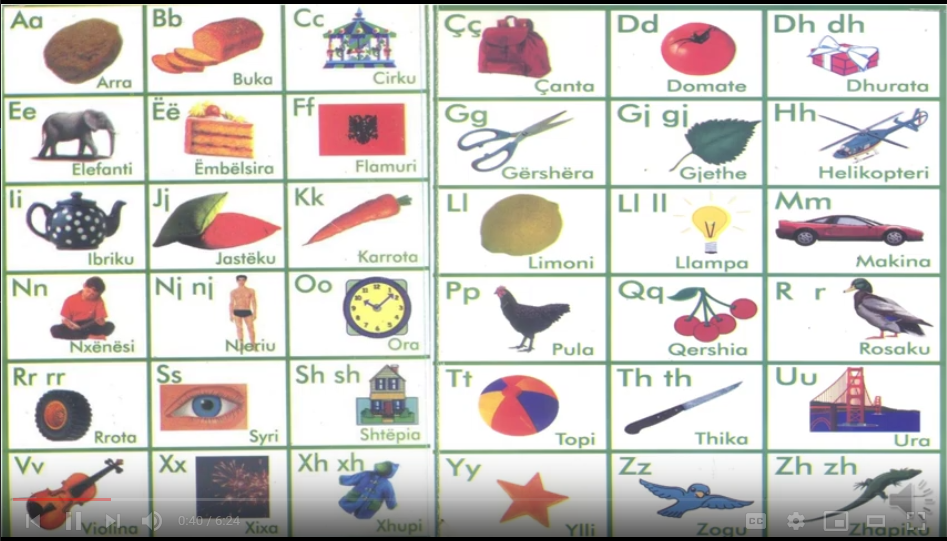
\includegraphics[width=0.8\textwidth]{src/images/alfabetoAlbanese.PNG}
    \caption{Alfabeto albanese}
\end{figure}

\chapter{L'essenziale nella comunicazione base}

\section{Saluti}

\begin{table}[ht]
    \centering
    \begin{tabular}{lr}
        \toprule
        Italiano    &   Albanese \\
        \midrule
        \addTranslationRow{Buon Mattino}\\
        \addTranslationRow{Buon pomeriggio}\\
        \addTranslationRow{Buona sera}\\
        \addTranslationRow{Buona notte}\\
        \addTranslationRow{A presto}\\
        \addTranslationRow{Piacere}\\
        \addTranslationRow{Ci vediamo presto}\\
        \addTranslationRow{Arrivederci}\\
        \addTranslationRow{Addio}\\
        \addTranslationRow{Ciao}\\
        \addTranslationRow{Bene}\\
        \bottomrule
    \end{tabular}
\end{table}

\section{Espressioni comuni}

\begin{table}[ht]
    \centering
    \begin{tabular}{lr}
        \toprule
        Italiano    &   Albanese \\
        \midrule
        \addTranslationRow{Grazie}\\
        \addTranslationRow{Per favore}\\
        \addTranslationRow{Perdonami}\\
        \addTranslationRow{Mi dispiace}\\
        \addTranslationRow{Come stai?}\\
        \addTranslationRow{Puoi ripeterlo un'altra volta per favore?}\\
        \addTranslationRow{Parlo poco albanese}\\
        \addTranslationRow{Non parlo per niente l'albanese}\\
        \addTranslationRow{Non capisco}\\
        \addTranslationRow{Un momento per favore}\\
        \addTranslationRow{Ti prego, aspetta un minuto}\\
        \addTranslationRow{Si (ok)}\\
        \addTranslationRow{No}\\
        \addTranslationRow{Forse}\\
        \addTranslationRow{Quindi}\\
        \bottomrule
    \end{tabular}
\end{table}

\chapter{Grammatica albanese}

\section{Verbo essere e avere}

\begin{table}[ht]
    \centering
    \begin{tabular}{lr}
        \toprule
        Italiano    &   Albanese \\
        \midrule
        Io sono & Unë iam \\
        Tu sei & Ti je\\
        Egli è & Ai është\\
        Ella è & Ajo është\\
        Noi siamo & Ne jemi \\
        Voi siete & Ju jeni \\
        Essi sono & Ata jan \\
        Esse sono & Ato jan \\
        \bottomrule
    \end{tabular}
    \caption{Verbo essere nell'indicativo}
\end{table}

\begin{table}[ht]
    \centering
    \begin{tabular}{lr}
        \toprule
        Italiano    &   Albanese \\
        \midrule
        Io sono & Unë kam \\
        Tu sei & Ti ke\\
        Egli è & Ai ka\\
        Ella è & Ajo ka\\
        Noi siamo & Ne kemi \\
        Voi siete & Ju keni \\
        Essi sono & Ata kanë \\
        Esse sono & Ato kanë \\
        \bottomrule
    \end{tabular}
    \caption{Verbo avere nell'indicativo}
\end{table}

\section{Verbi}

Ci sono 3 coniugazioni, che si distinguono per la terminazione dell'infinito presente.

\subsection{Prima Coniugazione}

Sono verbi il cui infinito termina con \dquote{j}.

\begin{table}[ht]
    \centering
    \begin{tabular}{lr}
        \toprule
        Italiano    &   Albanese \\
        \midrule
        \addTranslationRow{Andare}\\
        \addTranslationRow{Lavorare}\\
        \addTranslationRow{Imparare}\\
        \addTranslationRow{Vivere}\\
        \addTranslationRow{Cantare}\\
        \addTranslationRow{Leggere}\\
        \addTranslationRow{Scrivere}\\
        \addTranslationRow{Fare}\\
        \addTranslationRow{Ascoltare}\\
        \addTranslationRow{Capire}\\
        \addTranslationRow{Contare}\\
        \addTranslationRow{Dimenticare}\\
        \addTranslationRow{Guardare}\\
        \addTranslationRow{Iniziare}\\
        \addTranslationRow{Finire}\\
        \addTranslationRow{Pulire}\\
        \bottomrule
    \end{tabular}
    \caption{Verbo avere nell'indicativo}
\end{table}

Nella format dell'indicativo presente, i verbi sono coniugati in accordo alla \tblref{bl:verb:primaconiugazione:indicativo:presente}.

\begin{table}[ht]
    \centering
    \begin{tabular}{lr}
        \toprule
        Italiano    &   Albanese\\
        \midrule
        Io lavoro           &   Unë puno\textbf{j} \\
        Tu lavori           &   Ti puno\textbf{n} \\
        Egli/Ella lavora    &   Ai/Ajo puno\textbf{n} \\
        Noi lavoriamo       &   Ne puno\textbf{jmë} \\
        Voi lavorate        &   Ju puno\textbf{ni} \\
        Essi/esse lavorano  &   Ata/Ato puno\textbf{jnë} \\
        \bottomrule
    \end{tabular}
    \caption{indicativo presente, prima coniugazione.}
    \label{tbl:verb:primaconiugazione:indicativo:presente}
\end{table}

La stessa tabella è mostrata per il verbo andare (irregolare in italiano ma regolare in albanese).

\begin{table}[ht]
    \centering
    \begin{tabular}{lr}
        \toprule
        Italiano    &   Albanese\\
        \midrule
        Io vado           &   Unë shko\textbf{j} \\
        Tu vai           &   Ti shko\textbf{n} \\
        Egli/Ella va    &   Ai/Ajo shko\textbf{n} \\
        Noi andiamo       &   Ne shko\textbf{jmë} \\
        Voi andate        &   Ju shko\textbf{ni} \\
        Essi/esse vanno  &   Ata/Ato shko\textbf{jnë} \\
        \bottomrule
    \end{tabular}
    \caption{indicativo presente, prima coniugazione del verbo andare.}
    \label{tbl:verb:andare:primaconiugazione:indicativo:presente}
\end{table}

\subsection{Seconda Coniugazione}

Sono verbi il cui infinito termina con una qualunque consonante. Le più comuni sono \dquote{p}, \dquote{s}, \dquote{l}. Inoltre la radice dei verbi non è tutto l'infinito tranne l'ultima consonanta, ma è possibile che la penultima lettera (solitamente una vocale) sia inclusa nella desinenza). La coniugazione è una delle più irregolari: per questo mostreremo le varie coniugazioni per ogni tempo.

\begin{table}[ht]
    \centering
    \begin{tabular}{lr}
        \toprule
        Italiano    &   Albanese \\
        \midrule
        \addTranslationRow{Aprire}\\
        \addTranslationRow{Parlare}\\
        \addTranslationRow{Uscire}\\
        \addTranslationRow{Vendere}\\
        \addTranslationRow{Domandare}\\
        \addTranslationRow{chiamare}\\
        \addTranslationRow{bussare}\\
        \bottomrule
    \end{tabular}
    \caption{Verbi della seconda coniugazione}
\end{table}

A livello generico, la coniugazione segue la seguente forma:

\begin{table}[ht]
    \centering
    \begin{tabular}{lr}
        \toprule
        Italiano    &   Albanese\\
        \midrule
        Io          &   forma infinita \\
        Tu          &   forma infinita o \textbf{et} \\
        Egli/Ella   &   format infinita o \textbf{et} \\
        Noi         &   \textbf{im} \\
        Voi         &   \textbf{ni} \\
        Essi/esse   &   \textbf{in} \\
        \bottomrule
    \end{tabular}
    \caption{indicativo presente, seconda coniugazione di un generico verbo. Nella seconda colonna è mostrata la desinenza o, in caso di irregolarità, se è possibile usare anche la forma infinita del verbo.}
    \label{tbl:verb:secondaconiugazione:indicativo:presente}
\end{table}

\begin{table}[ht]
    \centering
    \begin{tabular}{lccccccc}
        \toprule
        Pronome     &   Aprire  & Parlare   & Uscire    & Vendere   & Domandare & chiamare & Bussare \\
        \midrule
        Io          &   hap     & flas      & dal       & shes      & pyes  & thërras   & trokas\\
        Tu          &   hap     & flet      & del       & shet      & pyes  & thërret   & troket\\
        Egli/Ella   &   hap     & flet      & del       & shet      & pyes &    thërret & troket\\
        Noi         &   hapim   & flasim    & dalim     & shesim    & pyesim    & thërrasim & trokasim\\
        Voi         &   hapni   & flisni    & dilni     & shisni    &pyesni     & thërrisni & trokisni\\
        Essi/esse   &   hapin   & flasin    & dalin     & shesin    & pyesin    & thërrasin & trokasin\\
        \bottomrule
    \end{tabular}
    \caption{indicativo presente, seconda coniugazione dei verbi hap, flas, dal, shes, pyes, thërras, trokas.}
    \label{tbl:verb:secondaconiugazione:indicativo:presente}
\end{table}

\subsection{Terza Coniugazione}

I verbi della terza coniugazione sono quelli i cui infinito termina con una vocale. Tra le vocali ammesse, troviamo \dquote{i}, \dquote{a}, e \dquote{e}. La coniugazione è sicuramente più regolare rispetto alla seconda. A livello generico la coniugazione si comporta come segue:

\begin{table}[ht]
    \centering
    \begin{tabular}{lr}
        \toprule
        Italiano    &   Albanese\\
        \midrule
        Io          &   forma infinita \\
        Tu          &   forma infinita\\
        Egli/Ella   &   format infinita\\
        Noi         &   \textbf{më} \\
        Voi         &   \textbf{ni} \\
        Essi/esse   &   \textbf{në} \\
        \bottomrule
    \end{tabular}
    \caption{indicativo presente, seconda coniugazione di un generico verbo. Nella seconda colonna è mostrata la desinenza o, in caso di irregolarità, se è possibile usare anche la forma infinita del verbo.}
    \label{tbl:verb:secondaconiugazione:indicativo:presente}
\end{table}

Una lista dei verbi è disponibile in \tblref{fig:verb:terzacongiugazione}.

\begin{table}[ht]
    \centering
    \begin{tabular}{lr}
        \toprule
        Italiano    &   Albanese \\
        \midrule
        \addTranslationRow{Restare}\\
        \addTranslationRow{Dormire}\\
        \addTranslationRow{Bere}\\
        \addTranslationRow{Conoscere}\\
        \addTranslationRow{Mangiare}\\
        \bottomrule
    \end{tabular}
    \caption{Verbi della terza coniugazione}
    \label{fig:verb:terzacongiugazione}
\end{table}

Esempi di come sono coniugati i verbi sono mostrati in \tblref{tbl:verb:terzaconiugazione:indicativo:presente}

\begin{table}[ht]
    \centering
    \begin{tabular}{lccccccc}
        \toprule
        Pronome     &   Restare  & Dormire   & Bere    & Conoscere   & Mangiare \\
        \midrule
        Io          &   rri     & fle      & pi       & di      & ha\\
        Tu          &   rri     & fle      & pi       & di      & ha\\
        Egli/Ella   &   rri     & fle      & pi       & di      & ha \\
        Noi         &   rrimë   & flemë    & pimë     & dimë    & hamë \\
        Voi         &   rrini   & fleni    & pini     & dini    & hani \\
        Essi/esse   &   rrinë   & flenë    & pinë     & dinë    & hanë\\
        \bottomrule
    \end{tabular}
    \caption{indicativo presente, seconda coniugazione dei verbi rri, fle, pi, di, ha.}
    \label{tbl:verb:terzaconiugazione:indicativo:presente}
\end{table}

\section{Negazioni}

\dquote{Tu non hai nessuno} diventa \dquote{Ti \textbf{nuk} ke asnjë}.

\section{Interrogazioni}

Per dire \glsref{Chi} puoi usare \glsdesc{Chi}. Per esempio \dquote{chi sei?} si può tradurre con \dquote{Kush je?}

Per dire \glsref{Cosa} puoi usare \glsdesc{çfarë} (\eg{} \dquote{Cosa vuoi?} si può tradurre con \dquote{çfarë do?})

\glsref{Come} si traduce con \glsdesc{Come}.
\glsref{Dove} si traduce con \glsdesc{Dove} (Dove sei? si tradure con \dquote{Kui je?})

In generale questi avverbi interrogativi vanno sempre ad inizio frase.

\begin{table}[ht]
    \centering
    \begin{tabular}{lr}
        \toprule
        Italiano    &   Albanese \\
        \midrule
        \addTranslationRow{Chi}\\
        \addTranslationRow{Cosa}\\
        \addTranslationRow{Come}\\
        \addTranslationRow{Quando}\\
        \addTranslationRow{Quanto}\\
        \addTranslationRow{Dove}\\
        \addTranslationRow{Perché}\\
        \bottomrule
    \end{tabular}
    \caption{Avverbi interrogativi}
\end{table}

\section{Preposizioni, congiunzioni e complementi}

Le preposizioni sono le seguenti:

\begin{table}[ht]
    \centering
    \begin{tabular}{lr}
        \toprule
        Italiano    &   Albanese \\
        \midrule
        \addTranslationRow{di (preposizione)}\\
        \addTranslationRow{a}\\
        \addTranslationRow{da}\\
        \addTranslationRow{in (preposizione)}\\
        \addTranslationRow{con}\\
        \addTranslationRow{su}\\
        \addTranslationRow{per}\\
        \addTranslationRow{tra/fra}\\
        \bottomrule
    \end{tabular}
    \caption{Le p}
\end{table}

Quese preposizioni sono solitamente messe dove in italiano verrebbero messe. Per esempio per dire \dquote{io vado a tirana} dico \dquote{Unë shkoj në Tiranë} (lascia perdere che anche Tirana è declinato).

Inoltre è interessante notare che mentre in italiano esistono 2 preposizioni \dquote{a} e \dquote{in} (per differenziare lo stato in luogo e moto al luogo), in albanese non c'è differenza tra le 2 e vengono entrambe tradotte con \gsldesc{in (preposizione)}.

Particolare attenzione va fatta alla preposizione \dquote{di}. Bisogna tradurre:

\begin{itemize}
    \item \dquote{di} con \dquote{i} quando il sostantivo che viene specificato dal complemento di specificazione è maschile;
    \item \dquote{di} con \dquote{e} quando il sostantivo che viene specificato dal complemento di specificazione è femminile;
\end{itemize}

Considera il seguente esempi: \dquote{il libro di Viola} e \dquote{il quaderno di Viola}. il Libro è \glsdesc{Libro} (in albanese maschile) mentre il Quaderno è \glsdesc{Quaderno} (in alòbanese femminile). La prima frase è tradotta con \dquote{Libri i Violës} (perché libri è maschile) mentre la seconda è tradotta con \dquote{Fletorja e Violës} (perché il quaderno è femminile): Il genere del complemento di specificazione (in questo caso Viola) non è coinvolto nella regola.

Ora, la domanda è: se io in italiano voglio usare un complemento, come lo dico in albanese? \tblref{tbl:complementi} ci dice cosa dobbiamo fare per esprimere un complemento in albanese


\begin{table}[ht]
    \centering
    \begin{tabular}{lcr}
        \toprule
        Italiano            & Domanda                   & Albanese \\
        \midrule
        \textbf{Oggetto}              & Chi? Che cosa?               &\\
        \textbf{Specificazione}      & Di chi? Di cosa?              &\\
        \textbf{termine}             & A chi? A cosa?                &\\
        \textbf{agente}              & in passivo: Da chi?           &\\
        \textbf{causa}               & per quale motivo?             &\\
        \textbf{stato in luogo}      & dove? in che luogo?           & në\\
        \textbf{moto a luogo}        & verso dove?                   &\\
        \textbf{moto da luogo}       & da dove?                      &\\
        \textbf{moto per luogo}      & attraverso dove?              &\\
        \textbf{tempo}               & quando?                       &\\
        \textbf{fine}                & al fine di chi? a che scopo?  &\\
        \textbf{mezzo/modo}          & per mezzo di chi? di che cosa?& në\\
        \textbf{compagnia}           & con chi? con che cosa?        & më\\
        \textbf{argomento}           & riguardo cosa?                &\\
        causa efficiente    & da chi? da cosa?              &\\
        prezzo              & per quanto?                   &\\
        abbondanza          & di che cosa?                  &\\
        unione              & con cosa?                     &\\
        qualità             & con quali caratteristiche?    &\\
        materia             & di cosa è composto?           &\\
        
        vantaggio           & In favore di chi? Di cosa?    &\\
        denominazione       & Di chi? Di cosa?              &\\
        limitazione         & relativamente a che cosa?     &\\
        provenienza         & da dove? da che cosa?         &\\
        paragone            & più o meno di chi? di cosa?   &\\
        età                 & a che età?                    &\\
        quantità            & in che quantità               &\\
        \bottomrule
    \end{tabular}
    \caption{Complementi}
    \label{tbl:complementi}
\end{table}

\section{Numeri}

\begin{note}
    L'albanese con i numero funziona tipo il francese: al posto di dire quaranta, usano 2 venti (proprio come in francese per dire 80 dicono quattro volte venti).
\end{note}

\begin{table}[ht]
    \centering
    \begin{tabular}{lr}
        \toprule
        Italiano     &   Albanese \\
        \midrule
        \addTranslationRow{Numero}\\
        \addTranslationRow{Zero}\\
        \addTranslationRow{Uno}\\
        \addTranslationRow{Due}\\
        \addTranslationRow{Tre}\\
        \addTranslationRow{Quattro}\\
        \addTranslationRow{Cinque}\\
        \addTranslationRow{Sei}\\
        \addTranslationRow{Sette}\\
        \addTranslationRow{Otto}\\
        \addTranslationRow{Nove}\\
        \addTranslationRow{Dieci}\\
        \addTranslationRow{Undici}\\
        \addTranslationRow{Dodici}\\
        \addTranslationRow{Tredici}\\
        \addTranslationRow{Quattordici}\\
        \addTranslationRow{Quindici}\\
        \addTranslationRow{Sedici}\\
        \addTranslationRow{Diciasette}\\
        \addTranslationRow{Diciotto}\\
        \addTranslationRow{Diciannove}\\
        \addTranslationRow{Venti}\\
        \addTranslationRow{Ventuno}\\
        \addTranslationRow{Ventidue}\\
        \addTranslationRow{Ventitre}\\
        \addTranslationRow{Ventiquattro}\\
        \addTranslationRow{Trenta}\\
        \addTranslationRow{Trentuno}\\
        \addTranslationRow{Trentadue}\\
        \addTranslationRow{Trentatre}\\
        \addTranslationRow{Trentaquattro}\\
        \addTranslationRow{Quaranta}\\
        \addTranslationRow{Cinquanta}\\
        \addTranslationRow{Sessanta}\\
        \addTranslationRow{Settanta}\\
        \addTranslationRow{Ottanta}\\
        \addTranslationRow{Novanta}\\
        \addTranslationRow{Cento}\\
        \addTranslationRow{Mille}\\
        \addTranslationRow{Centomila}\\
        \addTranslationRow{Un milione}\\
        \addTranslationRow{Dieci milioni}\\
        \bottomrule
    \end{tabular}
\end{table}

\chapter{Lessico Generico}

\section{Colori}

\begin{table}[ht]
    \centering
    \begin{tabular}{lr}
        \toprule
        Italiano    &   Albanese \\
        \midrule
        \addTranslationRow{Rosso}\\
        \addTranslationRow{Arancione}\\
        \addTranslationRow{Giallo}\\
        \addTranslationRow{Verde}\\
        \addTranslationRow{blu}\\
        \addTranslationRow{Viola}\\
        \addTranslationRow{rosa}\\
        \addTranslationRow{Bianco}\\
        \addTranslationRow{Marrone}\\
        \addTranslationRow{Grigio}\\
        \addTranslationRow{Nero}\\
        \addTranslationRow{Nera}\\
        \bottomrule
    \end{tabular}
\end{table}


\section{Giorni della settimana, mesi e stagioni}

\begin{table}[ht]
    \centering
    \begin{tabular}{lr}
        \toprule
        Italiano    &   Albanese \\
        \midrule
        \addTranslationRow{Sera}\\
        \addTranslationRow{Giorno}\\
        \addTranslationRow{Settimana}\\
        \addTranslationRow{Mese}\\
        \addTranslationRow{Anno}\\
        \addTranslationRow{Stagione}\\
        \addTranslationRow{Primavera}\\
        \addTranslationRow{Estate}\\
        \addTranslationRow{Autunno}\\
        \addTranslationRow{Inverno}\\
        \addTranslationRow{Finesettimana}\\
        \addTranslationRow{Lunedì}\\
        \addTranslationRow{Martedì}\\
        \addTranslationRow{Mercoledì}\\
        \addTranslationRow{Giovedì}\\
        \addTranslationRow{Venerdì}\\
        \addTranslationRow{Sabato}\\
        \addTranslationRow{Domenica}\\
        \addTranslationRow{Gennaio}\\
        \addTranslationRow{Febbraio}\\
        \addTranslationRow{Marzo}\\
        \addTranslationRow{Aprile}\\
        \addTranslationRow{Maggio}\\
        \addTranslationRow{Giugno}\\
        \addTranslationRow{Luglio}\\
        \addTranslationRow{Agosto}\\
        \addTranslationRow{Settembre}\\
        \addTranslationRow{Ottobre}\\
        \addTranslationRow{Novembre}\\
        \addTranslationRow{Dicembre}\\
        \bottomrule
    \end{tabular}
\end{table}

\section{A tavola}

\begin{table}[ht]
    \centering
    \begin{tabular}{lr}
        \toprule
        Italiano    &   Albanese \\
        \midrule
        \addTranslationRow{Pasta}\\
        \addTranslationRow{Risotto}\\
        \bottomrule
    \end{tabular}
    \caption{Primi}
\end{table}

\begin{table}[ht]
    \centering
    \begin{tabular}{lr}
        \toprule
        Italiano    &   Albanese \\
        \midrule
        \addTranslationRow{Branzino}\\
        \addTranslationRow{Gamberetti}\\
        \addTranslationRow{Gamberi}\\
        \bottomrule
    \end{tabular}
    \caption{Pesci}
\end{table}

\begin{table}[ht]
    \centering
    \begin{tabular}{lr}
        \toprule
        Italiano    &   Albanese \\
        \midrule
        \addTranslationRow{Oliva}\\
        \addTranslationRow{Pomodoro}\\
        \addTranslationRow{Cetriolo}\\
        \addTranslationRow{Tuship}\\
        \bottomrule
    \end{tabular}
    \caption{Verdura}
\end{table}


\begin{table}[ht]
    \centering
    \begin{tabular}{lr}
        \toprule
        Italiano    &   Albanese \\
        \midrule
        \addTranslationRow{Caffe}\\
        \addTranslationRow{Acqua}\\
        \addTranslationRow{te}\\
        \bottomrule
    \end{tabular}
    \caption{Bevande}
\end{table}


\begin{table}[ht]
    \centering
    \begin{tabular}{lr}
        \toprule
        Italiano    &   Albanese \\
        \midrule
        \addTranslationRow{Toilet}\\
        \bottomrule
    \end{tabular}
    \caption{Luoghi}
\end{table}

% \begin{table}[ht]
%     \centering
%     \begin{tabular}{lr}
%         \toprule
%         Italiano    &   Albanese \\
%         \midrule
%         \bottomrule
%     \end{tabular}
% \end{table}
\clearpage


\backmatter

\printglossary[type={itan}]
\clearpage
%\printglossary[type={anit}]
%\clearpage

\bibliographystyle{unsrt}
\bibliography{src/bibs/biblio}
%to use multiple biblios
%\bibliography{src/bibs/csp, src/bibs/pathfinding}


\end{document}
